%!TEX root = ../main.tex
% file: problem1.tex
\section{Animation of All Simple Paths of an Adjacency Matrix} % (fold)
\label{sec:animation_of_all_simple_paths_of_an_adjacency_matrix}
In the final problem we wish to extend the previous problem with an animating GUI which shows the possible simple paths one may take from one vertex to another. The path must include all paths up to length $n+1$ where $n$ is the number of vertices specified by the user.\\\\
There exist multiple algorithms which are able to solve for the paths between two vertices. The Floyd-Warshall algorithm is one which may find the shortest path between two vertices. It may be augmented to reconstruct all possible paths without repetition. Rather than implementing the aforementioned algorithm, it was decided to search for a scientific package which makes use of the algorithm. After a quick search on the Python website, a scientific package called \emph{NetworkX} was located, which specializes in network graphing. The method \emph{all\_simple\_paths} is able to give us all paths with no repeated nodes between a source and target node (\url{http://networkx.lanl.gov/preview/reference/generated/networkx.algorithms.simple_paths.all_simple_paths.html}).

\subsection{Program Description} % (fold)
\label{sub:program_description4}
We begin by ensuring that our class extends Problem 3's \emph{App} instance. We are then able to inherit all information from the previous GUI and need only to add additional functionality.
\begin{lstlisting}[caption={Inheritance of Problem 4}, label=lst:inherit,firstnumber=5]
class App3(App):
\end{lstlisting}\noindent
We see that our class \emph{App3} inherits \emph{App}. 
\begin{lstlisting}[caption={Initialization of Problem 3}, label=lst:initp3,firstnumber=12]
    prob3 = self.prob3 = App(master)
\end{lstlisting}\noindent
Prior to being able to use any information from Problem 3, we must initialize it as shown in Listing \ref{lst:initp3}. We set it to a class and local variable (although it is not necessary to create a local variable, it was done for simplicity). Now all routines from Problem 3 are available to Problem 4 as \emph{self.prob3.VARIABLE} or \emph{self.prob3.METHOD(VARIABLE)}.
\begin{lstlisting}[caption={Main Logic}, label=lst:main4,firstnumber=30]
    def animate(self):
        """animation main loop"""
        #localize the matrix
        try:
            self.matrix = numpy.copy(self.prob3.conMat)
        except:
            tkMessageBox.showerror('Usage Error','You must first generate a gragh BEFORE animating it!')
        #generate the edges from the matrix
        self.genEdges()
        #check if the user points exist
        edgeExist = self.checkIfEdgeExist()
        #then do our stuff if they exist, othewise tell user they messed up
        if edgeExist:
            self.genPaths()
            self.drawLines()
        else:
            tkMessageBox.showerror('Value Error','You did not select a valid point, it does not have connections. Please select a different point!')
\end{lstlisting}\noindent
The main logic for our application is performed when the user presses the additional button as seen Listing \ref{lst:main4}. To ensure that an adjacency matrix exists we attempt to copy it using a try statement. This allows us to localize the data for easier use, but also ensures that we do not have a crash from the user attempting to operate on data which does not exist. The next step is to generate a list of edges from the matrix which may be used by \emph{NetworkX}. The method \emph{checkIfEdgeExist} sees whether the vertices the user input to the entry boxes has any connections prior to beginning the animation. It returns a boolean, which is then evaluated to see whether we can proceed or should warn the user they selected a bad vertex.\\\\
Once a good vertex is selected, we are able to generate all possible simple paths.

\begin{lstlisting}[caption={Path Generation}, label=lst:path,firstnumber=83]
    def genPaths(self):
        """
        Generates our list of possible paths between two nodes in the network.
        This routine takes advantage of the all_simple_paths feature of networkx.
        I attempted to use the Floyd Warshall algorithm to reconstruct the paths,
        but was unsucessful. Luckily, open source scientific software that solves
        the problem at hand exists
        """
        # check whether the user has network x
        try:
            import networkx as nx
        # tell them how to get it if they don't have it
        except:
            tkMessageBox.showerror('Missing Package','In order to use this feature you must install NetworkX from http://networkx.lanl.gov\nUse \'sudo easy_install networkx\' to install the package')
        
        # make G our graph
        G = nx.Graph()
        
        # add our edges to the graph
        G.add_edges_from(self.edges)
        
        # generate our paths using all_simple_paths
        # http://networkx.lanl.gov/reference/generated/networkx.algorithms.simple_paths.all_simple_paths.html
        paths = nx.all_simple_paths(G, source=int(self.vEntry1.get()), target=int(self.vEntry2.get()), cutoff=self.n)
        # bring it back to list format so it can be used
        self.paths = list(paths)
\end{lstlisting}\noindent
Listing \ref{lst:path} shows the use of \emph{NetworkX} and our methods to generate a list of paths. We first try to import the \emph{NetworkX} package, if it is not available we inform the user how to get it. We then create a graph object, $G$. We add the edges calculated in the method \emph{genEdges} to the graph. We then use the method \emph{all\_simple\_paths} from the \emph{NetworkX} package to find all paths from the users source vertex to the users target vertex. The specified cutoff is the maximum length of the path. Since the method is a generator object, we must turn it into a list before it is usable.\\\\
Once the paths are known we animate lines between the vertices for each path. These are drawn in different colors per path based on a dictionary of colors that is specified in the script.
% subsection program_description (end)
\subsection{Results} % (fold)
\label{sub:results4}
It is rather difficult to display the results of Problem 4 in the paper, so it is recommended to run the script to see its performance. However, we shall show the functionality of the GUI.\\\\\\
\begin{figure}[H]
    \centering
        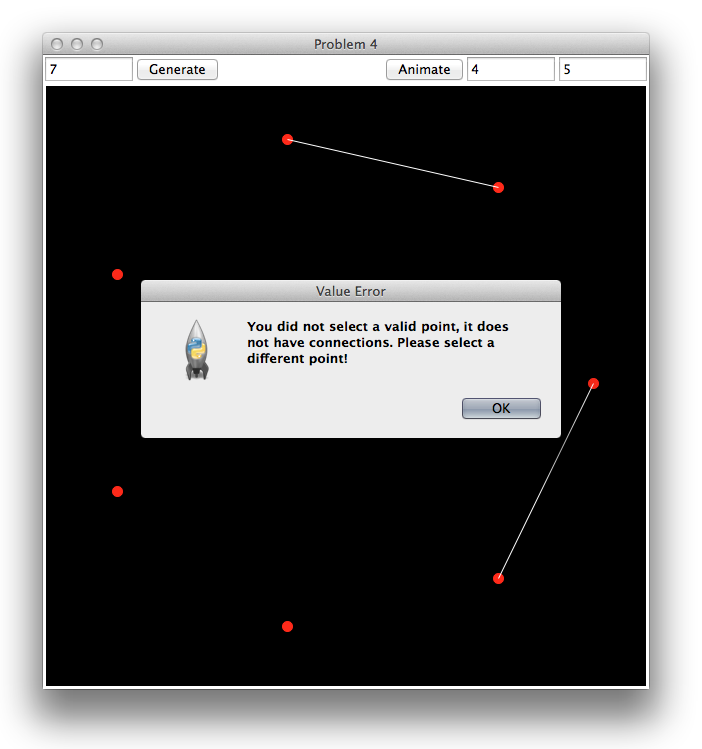
\includegraphics[width=4.75in,trim=1in .6in 1in 1in]{include/prob4invalid.png}
    \caption{Invalid Vertex Selection}
    \label{fig:include_prob4invalid}
\end{figure}
In Fig. \ref{fig:include_prob4invalid} we show the handling of bad vertices. If the user specifies vertices which have no edges then it returns a Value Error. This is done to prevent \emph{NetworkX} from crashing if it is given bad node values.

\begin{figure}[H]
    \centering
        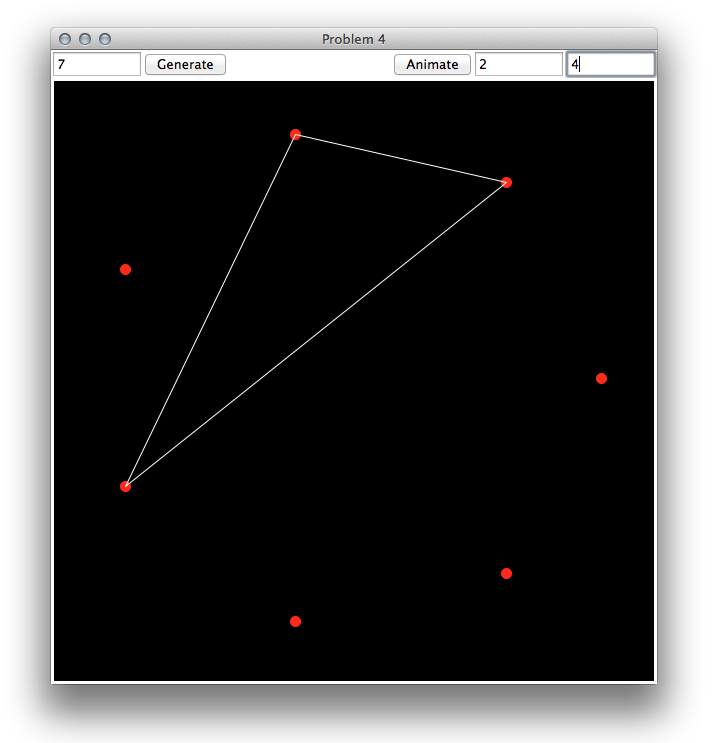
\includegraphics[width=4.75in,trim=1in .6in 1in 1in]{include/prob4before.png}
    \caption{Drawing of Edges Between Vertices}
    \label{fig:include_prob4before}
\end{figure}
In Fig. \ref{fig:include_prob4before} we show a simple case where two vertices have two possible paths between them. There are a total of 3 edges. We then find our paths.

\begin{figure}[H]
    \centering
        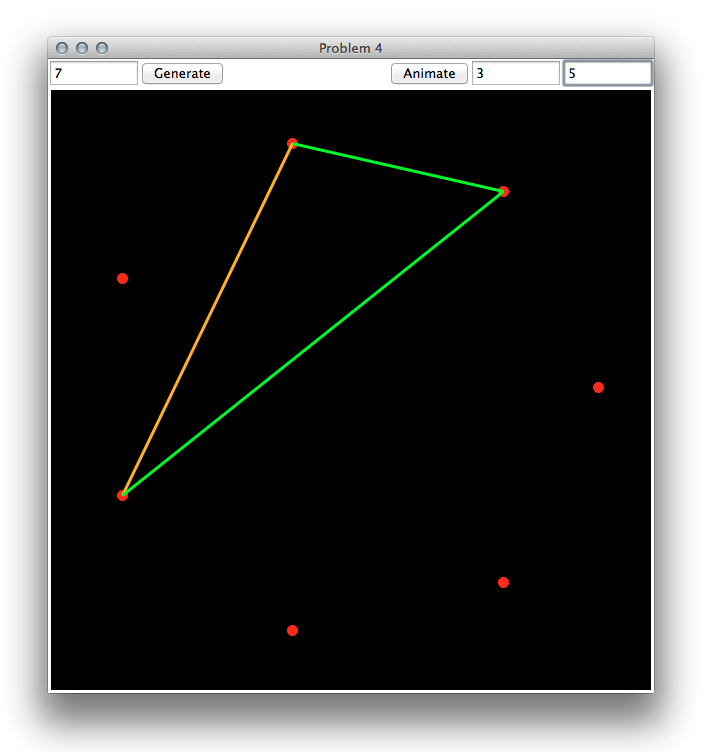
\includegraphics[width=4.75in,trim=1in .6in 1in 1in]{include/prob4paths.png}
    \caption{Calculated Paths Between Two Vertices}
    \label{fig:include_prob4paths}
\end{figure}
In Figure \ref{fig:include_prob4paths} we see the two possible paths between the two vertices outlined. Each possible path is assigned a different color, in this case orange and green. Although it is not possible to show the animation of the paths in images, allow me to assure the reader that the script highlights one edge at a time between two vertices. There is a delay specified between the drawing of the lines to produce the animation.

% subsection results4 (end)
% section animation_of_all_simple_paths_of_an_adjacency_matrix (end)